\documentclass[letterpaper,11pt]{article}

\setlength{\voffset}{0.1in}
\setlength{\paperwidth}{8.5in}
\setlength{\paperheight}{11in}
\setlength{\headheight}{0in}
\setlength{\headsep}{0in}
\setlength{\textheight}{11in}
\setlength{\textheight}{9.5in}
\setlength{\topmargin}{-0.25in}
\setlength{\textwidth}{7in}
\setlength{\topskip}{0in}
\setlength{\oddsidemargin}{-0.25in}
\setlength{\evensidemargin}{-0.25in}

%\usepackage{fullpage}
\usepackage{shading}
%\textheight=9.0in
\pagestyle{empty}
\raggedbottom
\raggedright
\setlength{\tabcolsep}{0in}

\usepackage{hyperref}
\usepackage{CJKutf8}
\usepackage{picins}
\usepackage{graphicx}
%-----------------------------------------------------------
%Custom commands
\newcommand{\resitem}[1]{\item #1 \vspace{-2pt}}
\newcommand{\resheading}[1]{{\large \parashade[.9]{sharpcorners}{\textbf{#1 \vphantom{p\^{E}}}}}}
\newcommand{\ressubheading}[4]{
\begin{tabular*}{6.5in}{l@{\extracolsep{\fill}}r}
		\textbf{#1} & #2 \\
		\textit{#3} & \textit{#4} \\
\end{tabular*}\vspace{-6pt}}
%-----------------------------------------------------------


\begin{document}
\begin{CJK}{UTF8}{hei}

\begin{tabular*}{7in}{l@{\extracolsep{\fill}}r}
\textbf{\Large 盛 艳}  & 13813147410\\
\#江苏省扬州大学 &  shengyan1985-at-gmail.com \\
信息工程学院 & http://liz.appspot.com\\
\end{tabular*}
\\

\vspace{0.1in}

\resheading{基本资料}

\parpic[r]{
  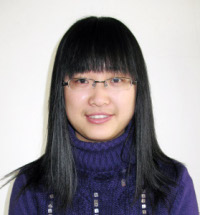
\includegraphics[height=5cm]{mypic.png}}
  
\begin{itemize}
\item
\item {} 
性别: 女

\item {} 
出生年月: 1985年8月

\item {} 
籍贯: 苏州

\item {} 
健康状况: 良好

\item {} 
毕业院校: \href{http://www.yzu.edu.cn}{扬州大学} 信息工程学院

\item {} 
专业/方向: 计算机应用技术/数据挖掘

\item {} 
通信地址: 江苏省扬州大学信息工程学院400173\#
\end{itemize}


\resheading{教育经历}
\begin{itemize}
\item
	\ressubheading{硕士阶段}{}{}{2007年9月 - 现在}
	\begin{itemize}
		\resitem{	以优异成绩推荐免试于扬州大学信息工程学院, 攻读计算机应用技术专业/数据挖掘方向硕士学位;}
		\resitem{完成基础课程的学习, 主要有: 矩阵论, 数据仓库, 数据挖掘, 分布式数据库原理, 并行处理技术, 并行算法设计与分析, 计算机体系结构, 计算机网络技术, 最优化理论;}
		\resitem{同时进行相关理论研究工作, 主要关于文本数据挖掘, 概念格相关方向, 熟悉多种数据挖掘算法及理论, 如: 经典Apriori, Decision Tree分类, 朴素贝叶斯分类, KNN分类, KMeans聚类, Rough Set Theory, Fuzzy Set Theory及形式概念分析中的Godin, Bordat算法等;}
		\resitem{目前已发表多篇国内/国际学术论文, 并于2009年8月中旬参加ICNC-FSKD'09国际学术会议交流.}
	\end{itemize}
\item
	\ressubheading{本科阶段}{}{}{2003年9月 - 2007年7月}
	\begin{itemize}
		\resitem{	于扬州大学信息工程学院, 攻读计算机科学与技术(师范)专业学士学位;}
		\resitem{认真学习各门基础课程, 主要有: 高等数学, 离散数学, 概率论与数理统计, 线性代数, PASCAL语言程序设计, C语言程序设计, C++程序设计, 汇编语言, 数据结构, 操作系统原理, 计算方法, 计算机通信, 编译原理, 数据库原理及应用, 面向对象技术, 计算机网络, 软件工程, 多媒体技术, 人工智能, 数字图像处理, 计算机组成原理, 微机原理, 单片机原理等, 取得优异成绩; 参加过2006年的ACM竞赛;}
		\resitem{期间, 自学了Photoshop, Illustrator等图像处理软件; 并对linux非常感兴趣, 从大三开始坚持使用linux操作系统(主要是ubuntu, fedora).}
	\end{itemize}

\end{itemize}

\resheading{技能}

\begin{description}
\item[语言:]
精通Python, C/C++, 熟悉 \LaTeX, Java, Pascal;
\item[操作系统:]
熟练使用Linux (Ubuntu, Fedora)的日常系统管理及维护;
\item[Web技术:]
熟悉Web应用开发; 熟练掌握Html, CSS, Javascript等Web技术, 并熟练使用 \href{http://jquery.com}{JQuery}, 有Ajax开发经验; 熟练掌握 \href{http://www.djangoproject.com/}{Django} 框架, 熟悉 \href{http://karrigell.sourceforge.net/}{Karrigell}, 熟悉GAE开发平台; 
\item[数据库技术:]
掌握 \href{http://www.mysql.com}{MySQL}, \href{http://www.sqlite.org}{Sqlite3} 等数据库使用;
\item[系统管理:]
熟悉 Apache, Lighttpd等web服务器配置和管理; 熟悉ftp, svn, trac, samba等常见服务配置;
\item[其他:]
Photoshop, Illustrator图形/图像处理; 
\item[英语水平:]
CET-4, 具有扎实的英语应用能力及较强的计算机专业英文文献阅读及翻译水平.
\end{description}

\resheading{项目经历}
\begin{itemize}

\item
	\ressubheading{Galicia平台扩展}{}{}{2007.9 - 2008.3}
	\begin{itemize}
		\resitem{	描述: Galicia是个开源项目, 在此基础上实现形式概念分析中的一些概念格构造算法, 如Godin算法, Godin改进算法等, 分析算法的时间空间复杂度.}
		\resitem{	职责: 在理解形式概念分析的基础上, 根据概念格自身特性, 掌握基本够格算法并实现, 之后图形显示结果格图, 以便更直观地得到概念格中概念及概念之间的继承关系.}
	\end{itemize}
	
\item
	\ressubheading{PR自动化工具}{}{}{2007.11 - 2008.3}
	\begin{itemize}
		\resitem{	描述: 由于学校的资料搜索系统涉及到很多脚本和程序文件数量很大, 为了使系统架构更加清晰, 也使开发维护人员更快更容易的理解整个流程, 设计并开发一个自动化脚本分析工具, 最大可能的呈现脚本, 程序, 配置文件之间的调用关系, 以便更好地理解整个系统.}
		\resitem{	职责: Linux下Python实现后台脚本并使用命令行带参数解析模式, 解析输入文件, 将产生的文件之间的调用关系录入Mysql数据库; 前端使用Django开发, 实现查询文件并输出相关的信息(包括该文件调用的c, perl, python, shell脚本, conf配置文件等的图像或文本信息).}
	\end{itemize}

\item
	\ressubheading{Openbookproject开放图书计划}{}{}{2008.4 - 2009.6}
	\begin{itemize}
		\resitem{	描述: 中文Pythonic技术图书的翻译编写项目, 其工程网址在 \href{http://code.google.com/p/openbookproject/}{http://code.google.com/p/openbookproject}. 其中的LovelyPython是原创图书, 将Python以最易懂的方式介绍给读者, 可作为Python初学者急速入门图书.}
		\resitem{	职责: 参与LovelyPython图书整个创作过程, 具体有: PCS环境篇/语法篇/模块篇中大多数章节的编写, 实例故事练习题设计及解答及各种校对等. 由于此项目是基于google code, 所以非常熟悉分布式团队合作的整个过程.}
	\end{itemize}

\item
	\ressubheading{禽流感病毒基因组生物信息学分析平台构建}{}{}{2008.11 - 2009.1}
	\begin{itemize}
		\resitem{	描述: 针对国际上各大生物信息中心提供的多个分析软件和基因/核酸数据库, 如BLAST检索系统(The Basic Local Alignment Search Tool, 一个基本的局部序列相似性比对搜索工具)及NCBI数据库(National Center for Biotechnology Information, 生物信息数据库中心), SMS2(The Sequence Manipulation Suite 2, 是用于分析较短的DNA和蛋白质序列的教学实验分析工具), Clustalx-2.0.10(用于进行DNA或蛋白质的多序列比对程序)等, 进行本地化生物信息学分析平台的构建, 并在此基础上进行功能扩展, 具体为禽流感病毒基因组数据库的选取, 定时更新及维护, 方便科研人员对禽流感病毒基因进行分析.}
		\resitem{	职责: 完整搭建生物信息分析平台及其扩展. 主要有: 服务器基础环境安装及部署, 采用RedHat Enterprise Linux 4.0 AS作为服务器操作系统, 采用Apache2.2作为Web服务器及相关支持工具的安装. BLAST分析工具的本地化部署及相关数据库的安装, SMS2和Clustalx的安装部署, 并将三者整合起来. 其中, 基于Django0.96进行信息平台扩展并使用mod\_python部署到Apache上形成一整套完整的分析系统. 对系统扩展的工作主要有: 在所有基因数据库中提取禽流感病毒基因并构建二级数据库, 随着NCBI数据库的更新也随之更新并提供扩展检索功能.}
	\end{itemize}

\item
	\ressubheading{eachdn交易平台}{}{}{2009.5 - 2009.9}
	\begin{itemize}
		\resitem{	描述: }
		\resitem{	职责: }
	\end{itemize}
	
\end{itemize}

\resheading{发表论文/书籍}
	\begin{tabular*}{6.5in}{l@{\extracolsep{\fill}}r}
		Yun Li, Yan Sheng, Luan Luan, Lianglei Sun and Ling Chen. A Personalized Search Results Ranking Method Based on WordNet. The 5th International Conference on Natural Computation(ICNC'09) and The 6th International Conference on Fuzzy Systems and Knowledge Discovery (FSKD'09), Tianjin, China;  & 2009\\
		Li Yun, Sheng Yan, Luan Luan. A Text Classification Method with an Effective Feature Extraction based on Category Analysis. The 5th International Conference on Natural Computation(ICNC'09) and The 6th International Conference on Fuzzy Systems and Knowledge Discovery (FSKD'09), Tianjin, China;  & 2009\\
		SHENG Yan, LI Yun, TIAN Su-fang, LUAN Luan. A Rough Concept Lattice Model of Variable Precision. IEEE International Symposium on Intelligent Information Technology Application 2008 (IITA'08), Shanghai City, China;   & 2008\\
		盛艳, 李云, 李拓, 栾鸾. 基于概念格模型的本体映射. 第三届江苏计算机大会(Jiangsu Computer Conference 2008, JSCC 2008); 此论文被评为第三届江苏计算机大会"优秀论文";  & 2008\\
		盛艳, 李云, 李拓, 袁运浩. 一种基于概念格模型的本体合并方法. 2008全国开放式分布与并行计算学术年会(DPCS2008);  & 2008\\
\end{tabular*}

\resheading{奖励/证书}
	\begin{tabular*}{6.5in}{l@{\extracolsep{\fill}}r}
		获一等专业奖学金   & 2003 - 2004学年\\
		被评为院"三好学生"  & 2003 - 2004学年\\
		获二等专业奖学金   & 2004 - 2005学年\\
		被评为校"三好学生" & 2004 - 2005学年\\
		获朱敬文奖学金  & 2005 - 2006学年\\
		获"优秀毕业生"称号  & 2007学年\\
		获研究生朱敬文奖学金  & 2007 - 2008学年\\
\end{tabular*}

\resheading{兴趣}

\begin{description}
\item[Academic:] Solid state devices,  nanotechnology, photonics, microcontrollers, RF/wireless
\item[Sports:] Playing hockey and swimming
\item[Computers:] Currently maintain two official Debian Linux packages, Mozilla beta tester, enjoy using and learning Linux systems, Building electronics projects at home, and writing JAVA software
\item[Musical:] Playing guitar and piano
\item[Membership:] Student member of IEEE since 1998, Materials Research Society member since 2002
\item[Other:] Reading novels
\end{description}

\end{CJK} 
\end{document}
